\chapter{Le cœur et la révolution cardiaque}\label{ch:b2:heart}

Prélevez le \omterm{def:b2:heart:anatomy}{cœur} d'une grenouille et plongez-le dans une solution
saline~: il continue de battre pendant des heures --- sans nerfs, sans
cerveau, sans \omterm{def:b2:blood-circulation:blood}{sang}, simple muscle qui se contracte de lui-même environ
une fois par seconde parce qu'un petit groupe de ses cellules ne peut pas
rester immobile. Un \omterm{def:b2:heart:anatomy}{cœur} humain fait cela quelque trois milliards de
fois au cours d'une vie, en déplaçant de l'ordre de deux cents millions
de litres, sans jamais être arrêté. Ce chapitre traite de cette pompe~:
ses cavités et ses valves, le cycle de remplissage et de vidange et les
pressions qui le commandent, le système électrique qui le rythme et la
trace qu'il laisse à la surface de la peau, la loi qui lui permet
d'ajuster à chaque battement son débit à ce qu'il reçoit, et les nerfs
et les hormones qui règlent sa fréquence et sa force.

\section{La pompe}

\begin{definition}[Cavités et valves]\label{def:b2:heart:anatomy}
\index{coeur@cœur}\index{oreillette}\index{ventricule}\index{valve cardiaque}
Le cœur est formé de deux pompes côte à côte, chacune composée d'une
\emph{oreillette}, qui reçoit le \omterm{def:b2:blood-circulation:blood}{sang} des \omterm{def:b2:blood-circulation:vessels}{veines}, et d'un
\emph{ventricule}, qui l'éjecte dans une \omterm{def:b2:blood-circulation:vessels}{artère}. Le cœur droit reçoit le
\omterm{def:b2:blood-circulation:blood}{sang} des \omterm{def:b2:blood-circulation:vessels}{veines} caves et l'envoie aux poumons par l'\omterm{def:b2:blood-circulation:vessels}{artère} pulmonaire~;
le cœur gauche le reçoit des \omterm{def:b2:blood-circulation:vessels}{veines} pulmonaires et l'envoie dans le corps
par l'aorte. Quatre valves rendent l'écoulement unidirectionnel~: les
\emph{valves auriculo-ventriculaires} (tricuspide à droite, mitrale à
gauche), des lames retenues par des cordages aux muscles papillaires
pour qu'elles ne soient pas refoulées dans l'oreillette~; et les
\emph{valves sigmoïdes} (pulmonaire et aortique), trois poches qui se
remplissent et se ferment lorsque la pression artérielle dépasse celle
du ventricule. Les valves sont passives~: elles s'ouvrent et se ferment
sous le seul effet des différences de pression. La paroi ventriculaire
est le \emph{myocarde}, un muscle strié fait de cellules ramifiées unies
bout à bout par des \emph{disques intercalaires} riches en jonctions
communicantes, si bien que le ventricule entier est électriquement une
seule cellule et se contracte d'un seul bloc~; la paroi du ventricule
gauche est trois fois plus épaisse que celle du droit, car il pompe
contre une pression cinq fois plus élevée. Le muscle cardiaque est
nourri par ses propres \emph{\omterm{def:b2:blood-circulation:vessels}{artères} coronaires}, qui se remplissent en
diastole, et il fonctionne presque entièrement en métabolisme aérobie
--- il ne peut pas s'endetter.
\end{definition}

\begin{omfigure}
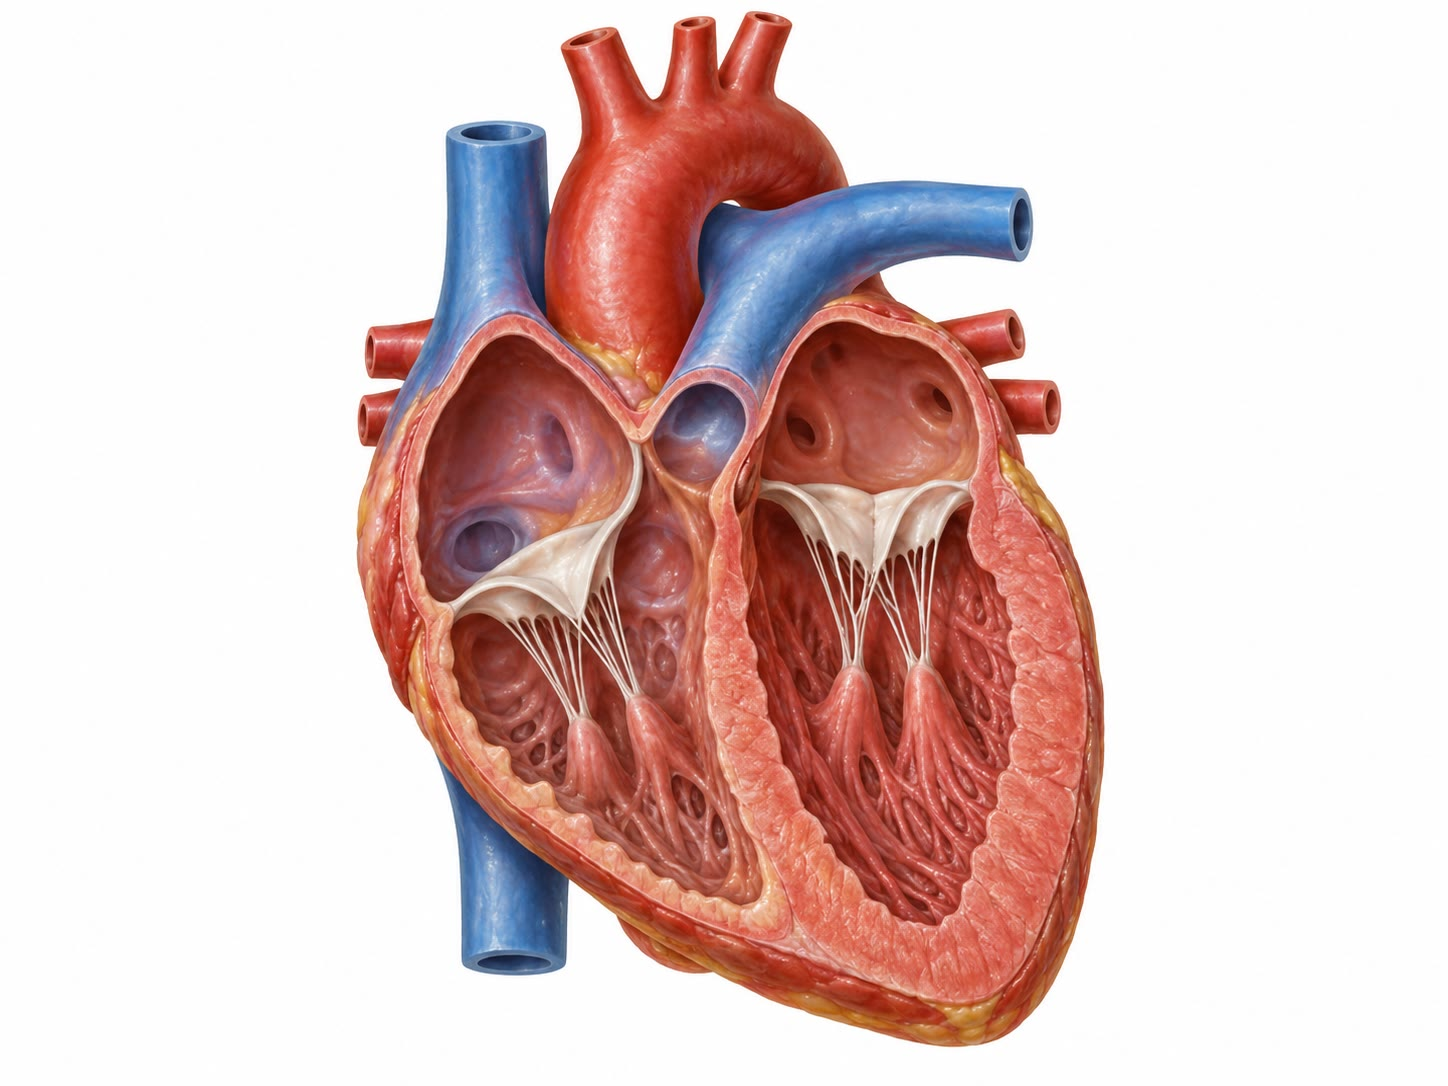
\includegraphics[width=0.55\linewidth]{images/book4/ai/b4-17-heart-cutaway.jpg}

{\small Le \omterm{def:b2:heart:anatomy}{cœur} en coupe frontale~: deux \omterm{def:b2:heart:anatomy}{oreillettes} en haut, deux
\omterm{def:b2:heart:anatomy}{ventricules} en bas, l'épais \omterm{def:b2:heart:anatomy}{ventricule} gauche, les valves
auriculo-ventriculaires avec leurs cordages, et les deux grosses \omterm{def:b2:blood-circulation:vessels}{artères}
qui partent du sommet.}
\end{omfigure}

\begin{proposition}[La révolution cardiaque]\label{prop:b2:heart:cycle}
\index{revolution cardiaque@révolution cardiaque}\index{systole}\index{diastole}\index{volume d'ejection systolique@volume d'éjection systolique}\index{fraction d'ejection@fraction d'éjection}
Au repos, un battement dure environ \qty{0.8}{s}. \emph{Diastole}
(\qty{0.5}{s})~: les \omterm{def:b2:heart:anatomy}{ventricules} se relâchent, leur pression passe sous
celle des \omterm{def:b2:heart:anatomy}{oreillettes}, les valves auriculo-ventriculaires s'ouvrent et
le \omterm{def:b2:blood-circulation:blood}{sang} entre, surtout passivement, puis avec une dernière poussée due à
la contraction des \omterm{def:b2:heart:anatomy}{oreillettes}~; le \omterm{def:b2:heart:anatomy}{ventricule} termine la diastole en
contenant environ \qty{120}{mL} (le \emph{volume télédiastolique}).
\emph{Systole} (\qty{0.3}{s})~: les \omterm{def:b2:heart:anatomy}{ventricules} se contractent~; dès que
leur pression dépasse celle des \omterm{def:b2:heart:anatomy}{oreillettes}, les valves
auriculo-ventriculaires se ferment (le premier bruit du \omterm{def:b2:heart:anatomy}{cœur}, «~toum~»),
et pendant quelques centièmes de seconde le \omterm{def:b2:heart:anatomy}{ventricule} comprime une
cavité close --- c'est la \emph{contraction isovolumétrique} --- jusqu'à
ce que sa pression dépasse la pression artérielle (\qty{80}{mmHg} à
gauche)~; les valves sigmoïdes s'ouvrent alors et le \omterm{def:b2:blood-circulation:blood}{sang} est éjecté. Le
\omterm{def:b2:heart:anatomy}{ventricule} gauche atteint \qty{120}{mmHg} et expulse environ
\qty{70}{mL} (le \emph{\omterm{prop:b2:heart:cycle}{volume d'éjection systolique}}, soit une
\emph{\omterm{prop:b2:heart:cycle}{fraction d'éjection}} de \qty{60}{\%})~; en se relâchant, sa
pression passe sous celle de l'aorte, la valve aortique claque (le
second bruit, «~ta~»), et une relaxation isovolumétrique ramène la
pression au niveau de celle de l'\omterm{def:b2:heart:anatomy}{oreillette}, moment où le remplissage
reprend. Le \omterm{def:b2:heart:anatomy}{cœur} droit fait de même à une pression cinq fois plus
faible, en éjectant le même volume.
\end{proposition}

\begin{omfigure}
\begin{tikzpicture}
\begin{axis}[
  width=0.9\linewidth, height=7.2cm,
  axis x line=bottom, axis y line=left,
  xmin=0, xmax=0.8, ymin=0, ymax=130,
  xlabel={temps dans le cycle (s)}, ylabel={pression (\unit{mmHg})},
  xlabel style={font=\small, at={(axis description cs:0.5,-0.1)}, anchor=north},
  ylabel style={font=\small},
  tick label style={font=\small}, xtick={0,0.1,0.3,0.8}, ytick={0,40,80,120},
  legend style={font=\scriptsize, at={(0.6,0.45)}, anchor=west, draw=none},
  clip=false,
]
% aortic pressure
\addplot[very thick, omThm] coordinates {(0,82) (0.05,80) (0.1,80) (0.12,95) (0.16,115) (0.2,120) (0.25,112) (0.3,100) (0.32,104) (0.34,100) (0.45,94) (0.6,88) (0.8,82)};
\addlegendentry{aorte}
% left ventricular pressure
\addplot[very thick, omDef] coordinates {(0,5) (0.04,8) (0.05,10) (0.08,60) (0.1,80) (0.12,95) (0.16,115) (0.2,120) (0.25,112) (0.3,100) (0.32,60) (0.35,20) (0.38,5) (0.5,3) (0.7,5) (0.75,8) (0.8,5)};
\addlegendentry{ventricule gauche}
% atrial pressure
\addplot[thick, omProp] coordinates {(0,6) (0.03,9) (0.06,6) (0.1,8) (0.15,6) (0.3,7) (0.36,10) (0.4,5) (0.6,6) (0.75,9) (0.8,6)};
\addlegendentry{oreillette gauche}
\draw[dashed, gray] (axis cs:0.05,0) -- (axis cs:0.05,128); \node[font=\scriptsize, anchor=south, align=center] at (axis cs:0.05,128) {fermeture\\mitrale};
\draw[dashed, gray] (axis cs:0.1,0) -- (axis cs:0.1,128); \node[font=\scriptsize, anchor=south, align=center] at (axis cs:0.13,128) {ouverture\\aortique};
\draw[dashed, gray] (axis cs:0.31,0) -- (axis cs:0.31,128); \node[font=\scriptsize, anchor=south, align=center] at (axis cs:0.31,128) {fermeture\\aortique};
\draw[dashed, gray] (axis cs:0.38,0) -- (axis cs:0.38,128); \node[font=\scriptsize, anchor=south, align=center] at (axis cs:0.4,128) {ouverture\\mitrale};
\node[font=\scriptsize] at (axis cs:0.2,45) {systole};
\node[font=\scriptsize] at (axis cs:0.55,25) {diastole};
\end{axis}
\end{tikzpicture}

{\small Les pressions dans le \omterm{def:b2:heart:anatomy}{cœur} gauche au cours d'un battement. Le
\omterm{def:b2:heart:anatomy}{ventricule} comprime une cavité close jusqu'à dépasser la pression
aortique, éjecte tant qu'il la dépasse, se relâche jusqu'à passer sous la
pression de l'\omterm{def:b2:heart:anatomy}{oreillette}, puis se remplit.}
\end{omfigure}

\begin{theorem}[Le travail du cœur]\label{thm:b2:heart:work}
\index{travail cardiaque}\index{boucle pression--volume}
Représenté dans le plan pression--volume, un battement du \omterm{def:b2:heart:anatomy}{ventricule}
gauche décrit une boucle --- remplissage le long du bas, contraction
isovolumétrique le long du côté droit, éjection le long du haut de
\qty{120}{mL} à \qty{50}{mL}, relaxation isovolumétrique le long du côté
gauche --- et l'aire de la boucle est le travail mécanique du
battement~:
\[
W = \oint P\,\mathrm{d}V \approx \bar P_{\text{éjection}}\times \text{volume d'éjection} \approx \qty{100}{mmHg}\times\qty{70}{mL} = \qty{0.93}{J}.
\]
À 72 battements par minute, le \omterm{def:b2:heart:anatomy}{ventricule} gauche fournit environ
\qty{1.1}{W}, le droit \qty{0.2}{W}~; le métabolisme du \omterm{def:b2:heart:anatomy}{cœur} est de
quelque \qty{8}{W}, si bien que son rendement mécanique est voisin de
\qty{15}{\%}, le reste étant de la chaleur et le coût du maintien de la
tension. Élever la pression contre laquelle pompe le \omterm{def:b2:heart:anatomy}{cœur} (hypertension,
valve aortique rétrécie) élève le travail par battement dans la même
proportion, et le muscle s'épaissit en réponse comme le fait tout muscle
--- jusqu'à ce que son irrigation coronaire ne puisse plus suivre son
volume.
\end{theorem}
\begin{proof}
Le travail est le produit d'une force par un déplacement et, pour une
pression agissant sur une paroi mobile, le produit de la pression par le
volume balayé~: $\mathrm{d}W = P\,\mathrm{d}V$. Sur une boucle fermée, le
travail net est l'aire enclose (le remplissage à basse pression coûte peu~;
l'éjection à haute pression rend beaucoup plus).
$\qty{100}{mmHg} = \qty{1.33e4}{Pa}$ et $\qty{70}{mL} =
\qty{7e-5}{m^3}$~: $1.33\times 10^{4}\times 7\times 10^{-5} =
\qty{0.93}{J}$~; multiplié par $1.2$ battement par seconde, \qty{1.1}{W}.
\end{proof}

\begin{omfigure}
\begin{tikzpicture}
\begin{axis}[
  width=0.62\linewidth, height=6cm,
  axis x line=bottom, axis y line=left,
  xmin=0, xmax=150, ymin=0, ymax=140,
  xlabel={volume du ventricule gauche (\unit{mL})}, ylabel={pression (\unit{mmHg})},
  xlabel style={font=\small, at={(axis description cs:0.5,-0.12)}, anchor=north},
  ylabel style={font=\small},
  tick label style={font=\small}, xtick={0,50,120}, ytick={0,80,120},
  clip=false,
]
\fill[omDef!12] (axis cs:50,5) -- (axis cs:120,8) -- (axis cs:120,80) -- (axis cs:110,115) -- (axis cs:80,122) -- (axis cs:50,100) -- cycle;
\draw[very thick, omDef, ->] (axis cs:50,5) -- (axis cs:120,8);
\draw[very thick, omDef, ->] (axis cs:120,8) -- (axis cs:120,80);
\draw[very thick, omDef, ->] (axis cs:120,80) .. controls (axis cs:110,118) and (axis cs:80,125) .. (axis cs:50,100);
\draw[very thick, omDef, ->] (axis cs:50,100) -- (axis cs:50,5);
\node[font=\scriptsize, anchor=south] at (axis cs:85,11) {remplissage};
\node[font=\scriptsize, anchor=west] at (axis cs:122,44) {contraction isovolumétrique};
\node[font=\scriptsize, anchor=south] at (axis cs:85,124) {éjection};
\node[font=\scriptsize, anchor=east] at (axis cs:48,52) {relaxation};
\node[font=\scriptsize] at (axis cs:85,60) {aire $=$ travail, \qty{0.9}{J}};
\end{axis}
\end{tikzpicture}

{\small La \omterm{thm:b2:heart:work}{boucle pression--volume} du \omterm{def:b2:heart:anatomy}{ventricule} gauche. L'aire enclose
est le travail d'un battement~; une pression artérielle plus élevée
élève le haut de la boucle, et le travail avec lui.}
\end{omfigure}

\section{L'horloge propre du cœur}

\begin{proposition}[Automatisme et conduction]\label{prop:b2:heart:conduction}
\index{noeud sinusal@nœud sinusal}\index{pacemaker}\index{noeud atrioventriculaire@nœud atrioventriculaire}\index{fibres de Purkinje}
Le battement naît dans le \emph{\omterm{prop:b2:heart:conduction}{nœud sinusal}}, un amas de cellules
musculaires spécialisées de la paroi de l'\omterm{def:b2:heart:anatomy}{oreillette} droite dont le
potentiel de membrane n'est jamais au repos~: après chaque potentiel
d'action, il remonte lentement (un \emph{potentiel pacemaker}, dû à un
courant sodique qui s'active aux potentiels négatifs et à des canaux
calciques) jusqu'à atteindre le seuil et déclencher un nouveau
potentiel d'action, une centaine de fois par minute si on le laisse
faire. L'influx se propage dans le muscle des \omterm{def:b2:heart:anatomy}{oreillettes}, de cellule en
cellule par les jonctions communicantes, et les \omterm{def:b2:heart:anatomy}{oreillettes} se
contractent~; il atteint le \emph{\omterm{prop:b2:heart:conduction}{nœud atrioventriculaire}}, seul pont
électrique entre \omterm{def:b2:heart:anatomy}{oreillettes} et \omterm{def:b2:heart:anatomy}{ventricules}, qui conduit lentement et le
retarde d'un dixième de seconde --- le temps pour les \omterm{def:b2:heart:anatomy}{oreillettes}
d'achever le remplissage des \omterm{def:b2:heart:anatomy}{ventricules}~; puis il dévale le
\emph{faisceau de His} et les \emph{\omterm{prop:b2:heart:conduction}{fibres de Purkinje}}, cellules à
conduction rapide qui le distribuent à tout le muscle ventriculaire en
\qty{30}{ms}, si bien que les \omterm{def:b2:heart:anatomy}{ventricules} se contractent de la pointe
vers la base, d'un seul bloc, et chassent le \omterm{def:b2:blood-circulation:blood}{sang} vers les valves de
sortie. Chaque partie de ce système peut imposer seule un rythme, chacune
plus lentement que la précédente (le \omterm{prop:b2:heart:conduction}{nœud sinusal} à 100, le \omterm{prop:b2:heart:conduction}{nœud
atrioventriculaire} à 50, les \omterm{prop:b2:heart:conduction}{fibres de Purkinje} à 30)~: si le \omterm{prop:b2:heart:conduction}{nœud
sinusal} défaille, un centre inférieur prend le relais --- à un rythme
plus lent.
\end{proposition}
\begin{proof}[Faits expérimentaux]
Un \omterm{def:b2:heart:anatomy}{cœur} isolé, ou une bandelette de tissu sinusal, bat dans une boîte
sans nerfs~; une bandelette de \omterm{def:b2:heart:anatomy}{ventricule} bat aussi, mais plus
lentement. Refroidir ou réchauffer le seul \omterm{prop:b2:heart:conduction}{nœud sinusal} modifie la
fréquence du \omterm{def:b2:heart:anatomy}{cœur} entier~; sectionner le faisceau atrioventriculaire
dissocie les \omterm{def:b2:heart:anatomy}{ventricules}, qui battent alors à leur propre rythme lent
tandis que les \omterm{def:b2:heart:anatomy}{oreillettes} continuent au rythme du nœud (bloc
auriculo-ventriculaire). L'enregistrement d'une seule cellule du nœud
montre la lente dépolarisation diastolique qu'aucune cellule musculaire
ordinaire ne présente~; le blocage du courant pacemaker la ralentit.
\end{proof}

\begin{omfigure}
\begin{tikzpicture}[every node/.style={font=\scriptsize}, >=stealth]
  % simplified heart outline, scaled up
  \draw[thick, fill=omThm!6] (0,0) .. controls (-4.2,1.3) and (-3.8,5.4) .. (-1.3,5.8) .. controls (0,6.1) and (0.6,5.6) .. (1.3,5.8) .. controls (3.8,5.4) and (4.2,1.3) .. (0,0);
  \draw[thick] (-3.0,3.5) .. controls (-0.8,3.85) and (0.8,3.85) .. (3.0,3.5);
  \draw[thick] (0,3.75) -- (0,0.6);
  \node at (-1.5,4.7) {oreillette droite}; \node at (1.5,4.7) {oreillette gauche};
  \node[align=center] at (-1.3,2.55) {ventricule\\droit}; \node[align=center] at (1.3,2.55) {ventricule\\gauche};
  % SA node
  \fill[omDef] (-2.5,5.0) circle (0.16); \node[omDef, anchor=east] at (-3.3,5.4) {nœud sinusal}; \draw[omDef] (-3.3,5.35) -- (-2.62,5.08);
  \draw[omDef, dashed] (-2.5,5.0) circle (0.45); \draw[omDef, dashed] (-2.5,5.0) circle (0.8);
  % AV node
  \fill[omDef] (-0.25,3.7) circle (0.14); \node[omDef, anchor=west] at (0.15,4.05) {nœud AV}; \draw[omDef] (0.15,4.05) -- (-0.12,3.78);
  % bundle and Purkinje
  \draw[very thick, omDef] (-0.25,3.6) -- (-0.25,2.1);
  \draw[very thick, omDef] (-0.25,2.1) .. controls (-0.8,1.4) .. (-1.9,1.1);
  \draw[very thick, omDef] (-0.25,2.1) .. controls (0.8,1.4) .. (1.9,1.1);
  \foreach \p in {(-1.9,1.1),(1.9,1.1)} { \draw[omDef] \p -- ++(-0.3,0.6); \draw[omDef] \p -- ++(0.3,0.7); \draw[omDef] \p -- ++(0,0.85); }
  \node[omDef, anchor=west] at (3.4,1.0) {fibres de Purkinje}; \draw[omDef] (3.4,1.0) -- (2.2,1.1);
  \node[omDef, anchor=east] at (-0.45,3.05) {faisceau de His};
  % timing
  \node[anchor=west, align=left] at (5.6,5.0) {décharge du nœud sinusal~: $t = 0$\\dépolarisation des oreillettes~: 0--\qty{80}{ms}};
  \node[anchor=west, align=left] at (5.6,3.5) {retard au nœud AV~: \qty{100}{ms}};
  \node[anchor=west, align=left] at (5.6,1.9) {faisceau et fibres de Purkinje~:\\ventricules dépolarisés\\à \qty{220}{ms}, pointe d'abord};
\end{tikzpicture}

{\small Le système de conduction. Le \omterm{prop:b2:heart:conduction}{nœud sinusal} se décharge, les
\omterm{def:b2:heart:anatomy}{oreillettes} se dépolarisent, le \omterm{prop:b2:heart:conduction}{nœud atrioventriculaire} retarde l'influx,
et le faisceau et les \omterm{prop:b2:heart:conduction}{fibres de Purkinje} le distribuent aux \omterm{def:b2:heart:anatomy}{ventricules}
de la pointe vers la base.}
\end{omfigure}

\begin{proposition}[L'électrocardiogramme]\label{prop:b2:heart:ecg}
\index{electrocardiogramme@électrocardiogramme}
Le \omterm{def:b2:heart:anatomy}{cœur} est une grande masse de cellules qui se dépolarisent et se
repolarisent en séquence, et les courants qui circulent dans le corps
autour de lui peuvent être enregistrés sous forme de tensions d'un
millivolt entre des électrodes placées sur les membres~: c'est
l'\emph{électrocardiogramme}. Ses ondes correspondent aux événements du
système de conduction~: l'\emph{onde P} est la dépolarisation des
\omterm{def:b2:heart:anatomy}{oreillettes}~; l'\emph{intervalle PR}, plat (\qty{0.16}{s}), est le
retard atrioventriculaire~; le \emph{complexe QRS}, pointu et bref
(\qty{0.08}{s}), est la dépolarisation ventriculaire --- ample parce que
la masse ventriculaire est grande, bref parce que les \omterm{prop:b2:heart:conduction}{fibres de Purkinje}
sont rapides~; l'\emph{onde T} est la repolarisation ventriculaire. (La
repolarisation des \omterm{def:b2:heart:anatomy}{oreillettes} est masquée par le QRS.) Le tracé
renseigne sur le rythme et la conduction, non sur la force~: un \omterm{prop:b2:heart:conduction}{nœud
atrioventriculaire} bloqué allonge l'intervalle PR ou dissocie P et QRS,
une région morte du \omterm{def:b2:heart:anatomy}{ventricule} déforme le QRS, une \omterm{def:b2:heart:anatomy}{oreillette}
désorganisée (fibrillation auriculaire) remplace les ondes P par un
bruit de fond et fait battre les \omterm{def:b2:heart:anatomy}{ventricules} irrégulièrement, et
l'intervalle entre deux ondes R donne la fréquence.
\end{proposition}

\begin{omfigure}
\begin{tikzpicture}
\begin{axis}[
  width=0.9\linewidth, height=5.2cm,
  axis x line=bottom, axis y line=left,
  xmin=0, xmax=1.0, ymin=-0.4, ymax=1.3,
  xlabel={temps (s)}, ylabel={mV},
  xlabel style={font=\small, at={(axis description cs:0.5,-0.12)}, anchor=north},
  ylabel style={font=\small},
  tick label style={font=\small}, xtick={0,0.2,0.4,0.6,0.8,1.0}, ytick={0,1},
  clip=false,
]
\addplot[very thick, omDef] coordinates {(0,0) (0.08,0) (0.1,0.05) (0.14,0.15) (0.18,0.05) (0.2,0) (0.28,0) (0.3,-0.1) (0.31,0) (0.33,1.1) (0.35,0) (0.36,-0.25) (0.375,0) (0.5,0) (0.54,0.1) (0.58,0.28) (0.62,0.1) (0.65,0) (0.88,0) (0.9,0.05) (0.94,0.15) (0.98,0.05) (1.0,0)};
\node[font=\scriptsize, anchor=south] at (axis cs:0.14,0.17) {P};
\node[font=\scriptsize, anchor=south] at (axis cs:0.33,1.12) {R};
\node[font=\scriptsize, anchor=north] at (axis cs:0.295,-0.11) {Q};
\node[font=\scriptsize, anchor=north] at (axis cs:0.365,-0.27) {S};
\node[font=\scriptsize, anchor=south] at (axis cs:0.58,0.3) {T};
\draw[<->, gray] (axis cs:0.1,0.45) -- (axis cs:0.3,0.45); \node[font=\scriptsize, anchor=south, gray] at (axis cs:0.2,0.46) {PR \qty{0.16}{s}};
\draw[<->, gray] (axis cs:0.3,0.6) -- (axis cs:0.375,0.6); \node[font=\scriptsize, anchor=west, gray] at (axis cs:0.38,0.6) {QRS \qty{0.08}{s}};
\draw[<->, gray] (axis cs:0.33,1.25) -- (axis cs:0.94,1.25); \node[font=\scriptsize, anchor=south, gray] at (axis cs:0.63,1.25) {intervalle R--R $=$ 60/fréquence};
\end{axis}
\end{tikzpicture}

{\small Un électrocardiogramme normal~: P (\omterm{def:b2:heart:anatomy}{oreillettes}), le retard PR au
\omterm{prop:b2:heart:conduction}{nœud atrioventriculaire}, QRS (dépolarisation ventriculaire), T
(repolarisation ventriculaire).}
\end{omfigure}

\section{La régulation du débit}

\begin{theorem}[La loi de Frank--Starling]\label{thm:b2:heart:starling}
\index{loi de Frank--Starling}\index{precharge@précharge}\index{debit cardiaque@débit cardiaque}
La force d'une contraction ventriculaire augmente avec le volume qui a
rempli le \omterm{def:b2:heart:anatomy}{ventricule}~: dans la plage de fonctionnement, plus le
\omterm{def:b2:heart:anatomy}{ventricule} est étiré en diastole (la \emph{précharge}), plus il éjecte en
systole. Le \omterm{def:b2:heart:anatomy}{cœur} expulse donc, battement après battement, tout ce qu'il
reçoit --- une hausse de \qty{20}{\%} du retour veineux entraîne une
hausse de \qty{20}{\%} du volume d'éjection sans aucun nerf ni aucune
hormone --- et les deux \omterm{def:b2:heart:anatomy}{ventricules}, qui doivent déplacer le même volume,
s'équilibrent automatiquement~: si le \omterm{def:b2:heart:anatomy}{cœur} droit envoie davantage de
\omterm{def:b2:blood-circulation:blood}{sang} aux poumons, le \omterm{def:b2:heart:anatomy}{cœur} gauche en reçoit davantage et pompe davantage.
Le mécanisme réside dans le \omterm{def:b2:cell-differentiation:fibre}{sarcomère}~: aux faibles longueurs d'un
\omterm{def:b2:heart:anatomy}{ventricule} mal rempli, les filaments épais et fins se chevauchent trop
et la sensibilité au calcium est basse~; l'étirement vers la longueur
optimale (\qty{2.2}{\micro m}) accroît à la fois le chevauchement
disponible pour les ponts actine-myosine et la sensibilité, si bien que
la même impulsion calcique produit plus de force. Au-delà de l'optimum
(un \omterm{def:b2:heart:anatomy}{cœur} distendu et défaillant), la force diminue de nouveau.
\end{theorem}
\begin{proof}[Faits expérimentaux]
Frank (1895) enregistra la pression développée par un \omterm{def:b2:heart:anatomy}{ventricule} de
grenouille rempli à différents volumes~: la pression maximale augmentait
avec le volume de remplissage jusqu'à un maximum, puis diminuait.
Starling (1914), sur une préparation cœur--poumons de chien dans laquelle
le retour veineux et la résistance artérielle pouvaient être réglés
indépendamment, montra qu'élever le retour élevait le débit battement
après battement, et qu'une élévation de la résistance artérielle était
compensée, après quelques battements d'accumulation, par un volume
télédiastolique plus grand et un débit rétabli --- le \omterm{def:b2:heart:anatomy}{ventricule} répond à
une charge en s'étirant, et à un étirement en se contractant plus fort.
\end{proof}

\begin{omfigure}
\begin{tikzpicture}
\begin{axis}[
  width=0.66\linewidth, height=5.4cm,
  axis x line=bottom, axis y line=left,
  xmin=0, xmax=200, ymin=0, ymax=140,
  xlabel={volume télédiastolique (\unit{mL})}, ylabel={volume d'éjection (\unit{mL})},
  xlabel style={font=\small, at={(axis description cs:0.5,-0.13)}, anchor=north},
  ylabel style={font=\small},
  tick label style={font=\small}, xtick={0,50,100,150,200}, ytick={0,50,100},
  legend style={font=\scriptsize, at={(0.5,-0.3)}, anchor=north, draw=none, legend columns=3},
  clip=false,
]
\addplot[very thick, omDef, domain=40:200, samples=60] {130*(1-exp(-(x-40)/70))};
\addlegendentry{normal}
\addplot[very thick, omThm, domain=40:200, samples=60] {130*1.3*(1-exp(-(x-40)/55))};
\addlegendentry{avec stimulation sympathique}
\addplot[very thick, omExo!70!black, domain=40:200, samples=60] {130*0.5*(1-exp(-(x-40)/90))};
\addlegendentry{cœur défaillant}
\fill[omDef] (axis cs:120,88) circle (2pt); \node[font=\scriptsize, anchor=south east] at (axis cs:118,90) {repos};
\end{axis}
\end{tikzpicture}

{\small Courbes de Starling. Le volume d'éjection augmente avec le
remplissage~; les nerfs sympathiques déplacent la courbe vers le haut
(plus de débit pour un même remplissage), un \omterm{def:b2:heart:anatomy}{cœur} défaillant la déplace
vers le bas.}
\end{omfigure}

\begin{proposition}[Nerfs et hormones]\label{prop:b2:heart:control}
\index{systeme nerveux sympathique!coeur@système nerveux sympathique!cœur}\index{nerf vague}\index{adrenaline@adrénaline}\index{debit cardiaque@débit cardiaque}
Le \omterm{thm:b2:heart:starling}{débit cardiaque} est le produit de la fréquence cardiaque par le
volume d'éjection~: \qty{5}{L/min} au repos, et jusqu'à \qty{25}{L/min}
chez un athlète entraîné à l'effort. Les deux facteurs sont fixés par
les nerfs autonomes. Le \emph{\omterm{prop:b2:heart:control}{nerf vague}} (parasympathique), en libérant
de l'acétylcholine sur le \omterm{prop:b2:heart:conduction}{nœud sinusal}, ralentit la dérive du
pacemaker et maintient la fréquence de repos à 70 au lieu des 100
propres au nœud~; si l'on sectionne les \omterm{prop:b2:heart:control}{nerfs vagues}, la fréquence
augmente. Les nerfs \emph{sympathiques}, en libérant de la
noradrénaline, et la médullosurrénale, en libérant de
l'\emph{adrénaline} dans le \omterm{def:b2:blood-circulation:blood}{sang}, accélèrent la dérive (plus de
battements), accélèrent la conduction et augmentent la force de
contraction pour tout remplissage (une courbe de Starling plus raide,
propriété appelée \emph{contractilité}), en augmentant le calcium
délivré aux \omterm{def:b2:cell-differentiation:fibre}{sarcomères} à chaque battement. À l'effort, le frein vagal
est d'abord relâché, puis l'accélérateur sympathique enfoncé, et une
fréquence de 180 avec un volume d'éjection de \qty{140}{mL} donne
\qty{25}{L/min}~; les signaux passent par les récepteurs et les seconds
messagers du \cref{ch:b2:cell-signalling}, et l'ensemble est commandé par
les centres régulateurs de la pression du
\cref{ch:b2:blood-pressure}.
\end{proposition}

\begin{example}[Lire un cœur]\label{ex:b2:heart:reading}
Deux bruits par battement~: «~toum~», la fermeture des valves
auriculo-ventriculaires au début de la systole~; «~ta~», la fermeture des
valves sigmoïdes à sa fin. Un souffle est un écoulement turbulent à
travers une valve rétrécie (une sténose) ou à rebours à travers une valve
qui fuit (une insuffisance)~: un souffle entre «~toum~» et «~ta~»
signale une valve mitrale qui fuit ou une valve aortique rétrécie, un
souffle après «~ta~» une valve aortique qui fuit. Un pouls de 70 avec une
pression artérielle de
$120/80$~mmHg correspond à un volume d'éjection voisin de \qty{70}{mL}~;
une fréquence de 40 chez un athlète traduit un grand volume d'éjection et
un fort tonus vagal~; une fréquence de 40 avec un intervalle PR qui
s'allonge jusqu'à ce qu'un battement saute signale un \omterm{prop:b2:heart:conduction}{nœud
atrioventriculaire} malade. La physiologie de ce chapitre est ce qu'un
médecin entend au stéthoscope en trente secondes.
\end{example}

\section{Exercices}

\begin{exercise}[$\star$]\label{exo:b2:heart:1}
Suivre une goutte de \omterm{def:b2:blood-circulation:blood}{sang} de la \omterm{def:b2:blood-circulation:vessels}{veine} cave à l'aorte, en nommant dans
l'ordre chaque cavité, chaque valve et chaque vaisseau.
\end{exercise}

\begin{exercise}[$\star$]\label{exo:b2:heart:2}
Donner les phases de la \omterm{prop:b2:heart:cycle}{révolution cardiaque} avec l'état de chaque valve
dans chaque phase, et l'événement à l'origine de chacun des deux bruits
du \omterm{def:b2:heart:anatomy}{cœur}.
\end{exercise}

\begin{exercise}[$\star$]\label{exo:b2:heart:3}
Nommer dans l'ordre les parties du système de conduction, avec le temps
que met l'influx pour atteindre chacune, et l'onde de
l'électrocardiogramme que produit chacune.
\end{exercise}

\begin{exercise}[$\star$]\label{exo:b2:heart:4}
Énoncer la \omterm{thm:b2:heart:starling}{loi de Frank--Starling} et dire pourquoi elle garantit que les
deux \omterm{def:b2:heart:anatomy}{ventricules} pompent le même volume.
\end{exercise}

\begin{exercise}[$\star\star$]\label{exo:b2:heart:5}
Un \omterm{def:b2:heart:anatomy}{cœur} a un volume télédiastolique de \qty{130}{mL} et un volume
télésystolique de \qty{50}{mL} à 70 battements par minute. Calculer le
volume d'éjection, la \omterm{prop:b2:heart:cycle}{fraction d'éjection} et le \omterm{thm:b2:heart:starling}{débit cardiaque}. Un \omterm{def:b2:heart:anatomy}{cœur}
défaillant a \qty{180}{mL} et \qty{120}{mL}~: refaire le calcul, et dire
ce qu'est devenue la \omterm{prop:b2:heart:cycle}{fraction d'éjection}.
\end{exercise}

\begin{exercise}[$\star\star$]\label{exo:b2:heart:6}
Calculer le travail d'un battement pour un volume d'éjection de
\qty{70}{mL} à une pression moyenne d'éjection de \qty{100}{mmHg}, et la
puissance à 72 battements par minute. Refaire le calcul pour un
hypertendu à \qty{150}{mmHg}. De combien de dioxygène supplémentaire par
minute le second \omterm{def:b2:heart:anatomy}{cœur} a-t-il besoin, si le rendement mécanique est de
\qty{15}{\%} et si \qty{1}{mL} de dioxygène fournit \qty{20}{J}~?
\end{exercise}

\begin{exercise}[$\star\star$]\label{exo:b2:heart:7}
Sur un électrocardiogramme, les ondes R sont espacées de \qty{0.5}{s}
dans un enregistrement et de \qty{1.5}{s} dans un autre. Donner les
fréquences cardiaques. Dans un troisième, les ondes P surviennent toutes
les \qty{0.6}{s} et les complexes QRS toutes les \qty{1.8}{s}, sans
relation fixe. Que s'est-il passé~?
\end{exercise}

\begin{exercise}[$\star\star$]\label{exo:b2:heart:8}
Le potentiel d'une cellule du \omterm{prop:b2:heart:conduction}{nœud sinusal} dérive de \qty{-60}{mV}
jusqu'à un seuil de \qty{-40}{mV} à raison de \qty{25}{mV/s}, avant
chaque potentiel d'action de \qty{0.15}{s}. Calculer l'intervalle entre
deux battements et la fréquence. L'acétylcholine abaisse la dérive à
\qty{18}{mV/s} et le potentiel de départ à \qty{-65}{mV}~; la
noradrénaline élève la dérive à \qty{40}{mV/s}. Calculer les deux
fréquences.
\end{exercise}

\begin{exercise}[$\star\star$]\label{exo:b2:heart:9}
Expliquer pourquoi le retard au \omterm{prop:b2:heart:conduction}{nœud atrioventriculaire} est nécessaire,
ce qu'il adviendrait du débit sans lui, et pourquoi un nœud lent (un long
intervalle PR) est inoffensif jusqu'à un certain point et dangereux
au-delà.
\end{exercise}

\begin{exercise}[$\star\star\star$]\label{exo:b2:heart:10}
Un athlète au repos a une fréquence de 45 et un débit de \qty{5}{L/min}~;
à l'effort, une fréquence de 180 et \qty{30}{L/min}. Calculer les volumes
d'éjection et dire ce qu'apportent respectivement la courbe de Starling
et les nerfs sympathiques. Pourquoi la fréquence ne peut-elle pas
utilement dépasser 200 environ~?
\end{exercise}

\begin{exercise}[$\star\star\star$]\label{exo:b2:heart:11}
Une valve aortique rétrécie laisse une ouverture de \qty{1}{cm^2} au lieu
de \qty{3}{cm^2}. À l'aide de la continuité, calculer la vitesse du \omterm{def:b2:blood-circulation:blood}{sang}
éjecté à \qty{250}{mL/s} à travers chacune, puis, à l'aide de la relation
de Bernoulli ($\Delta P = \tfrac12\rho v^2$), la pression que le
\omterm{def:b2:heart:anatomy}{ventricule} doit développer au-dessus de la pression aortique dans chaque
cas. Comment le \omterm{def:b2:heart:anatomy}{ventricule} y fait-il face, et quel en est le coût à
terme~?
\end{exercise}

\begin{exercise}[$\star\star\star$]\label{exo:b2:heart:12}
«~Le \omterm{def:b2:heart:anatomy}{cœur} est une pompe qui se régule elle-même et que le système
nerveux ne fait qu'ajuster.~» Discuter, en distinguant ce qu'apportent
respectivement l'automatisme, la \omterm{thm:b2:heart:starling}{loi de Frank--Starling} et les nerfs
autonomes, et ce que peut et ne peut pas faire un \omterm{def:b2:heart:anatomy}{cœur} transplanté ---
qui n'a pas de nerfs.
\end{exercise}

\section{Problème~: un cœur sous contrainte}

\begin{problem}[{Problème du week-end --- un même cœur suivi du repos à
l'effort puis dans la maladie~: sa révolution chronométrée, son travail
calculé, son électrocardiogramme lu, sa réponse de Starling et son
contrôle autonome quantifiés, et le coût d'une valve rétrécie estimé,
jusqu'au débit au repos et à l'effort, au travail par battement et au
gradient de pression à travers la sténose}]
\label{pb:b2:heart:1}
Données~: au repos, fréquence 70, volume télédiastolique \qty{130}{mL},
volume télésystolique \qty{60}{mL}, pression moyenne d'éjection
\qty{100}{mmHg} ($\qty{1}{mmHg} = \qty{133}{Pa}$), pression aortique
$120/80$~mmHg. La systole dure \qty{0.3}{s} quelle que soit la
fréquence. Pacemaker~: dérive de \qty{-60}{mV} à \qty{-40}{mV}, potentiel
d'action de \qty{0.15}{s}. Le \omterm{def:b2:heart:anatomy}{cœur} consomme \qty{20}{J} par millilitre
de dioxygène, avec un rendement mécanique de \qty{15}{\%}~; le \omterm{def:b2:blood-circulation:blood}{sang}
coronaire transporte \qty{0.2}{mL} de dioxygène par millilitre et le
\omterm{def:b2:heart:anatomy}{cœur} en extrait \qty{70}{\%}. Masse volumique du \omterm{def:b2:blood-circulation:blood}{sang}
\qty{1060}{kg/m^3}.

\medskip
\noindent\textbf{Partie I --- La révolution au repos.}
\begin{enumerate}
  \item Calculer le volume d'éjection, la \omterm{prop:b2:heart:cycle}{fraction d'éjection} et le \omterm{thm:b2:heart:starling}{débit
        cardiaque}.
  \item Calculer la durée d'un cycle et celle de la diastole.
  \item Calculer le débit moyen d'éjection pendant la systole, en
        millilitres par seconde, et la vitesse moyenne à travers une
        valve aortique de \qty{3}{cm^2}.
  \item La pression ventriculaire monte à raison de \qty{1500}{mmHg/s}
        pendant la contraction isovolumétrique, de 10 à \qty{80}{mmHg}.
        Combien de temps dure cette phase~?
  \item Calculer le travail d'un battement et la puissance mécanique du
        \omterm{def:b2:heart:anatomy}{ventricule} gauche.
  \item Calculer la puissance totale du \omterm{def:b2:heart:anatomy}{cœur} et sa consommation de
        dioxygène (les deux \omterm{def:b2:heart:anatomy}{ventricules}~: compter le droit pour un
        cinquième du gauche).
  \item Calculer le débit sanguin coronaire nécessaire pour fournir ce
        dioxygène.
\end{enumerate}

\medskip
\noindent\textbf{Partie II --- Le pacemaker et le tracé.}
\begin{enumerate}[resume]
  \item Quelle vitesse de dérive (\unit{mV/s}) donne une fréquence de 70~?
  \item Le \omterm{prop:b2:heart:control}{nerf vague} est sectionné~: la fréquence devient 100. Quelle
        vitesse de dérive cela représente-t-il~?
  \item Calculer la vitesse de dérive correspondant à une fréquence de
        180 à l'effort.
  \item Sur l'électrocardiogramme au repos, donner l'intervalle R--R, et
        dire à quoi correspondent les ondes P, QRS et T.
  \item L'intervalle PR vaut \qty{0.16}{s} au repos. Sa durée tient
        surtout au retard du \omterm{prop:b2:heart:conduction}{nœud atrioventriculaire}~: expliquer ce que
        permet ce retard et pourquoi une fréquence de 180 exige que le
        nœud accélère lui aussi.
  \item L'électrocardiogramme d'un patient montre des complexes QRS
        toutes les \qty{1.5}{s} et des ondes P toutes les \qty{0.8}{s},
        sans relation. Poser le diagnostic, donner la fréquence
        ventriculaire, et dire quel tissu rythme les \omterm{def:b2:heart:anatomy}{ventricules}.
\end{enumerate}

\medskip
\noindent\textbf{Partie III --- L'effort.}
À l'effort, la fréquence monte à 180 et les nerfs sympathiques
accroissent la contractilité, si bien que le volume télésystolique tombe
à \qty{30}{mL}~; le retour veineux porte le volume télédiastolique à
\qty{150}{mL}.
\begin{enumerate}[resume]
  \item Calculer le volume d'éjection, la \omterm{prop:b2:heart:cycle}{fraction d'éjection} et le
        débit.
  \item Calculer la durée de la diastole à 180 et expliquer pourquoi la
        fréquence ne peut pas utilement monter beaucoup plus haut.
  \item Calculer la puissance du \omterm{def:b2:heart:anatomy}{ventricule} gauche pour une pression
        moyenne d'éjection de \qty{120}{mmHg}, et la consommation de
        dioxygène du \omterm{def:b2:heart:anatomy}{cœur}.
  \item Calculer le débit coronaire nécessaire, et le comparer au repos.
        Pourquoi le raccourcissement de la diastole pose-t-il problème à
        ce débit~?
  \item Sans nerfs sympathiques (un \omterm{def:b2:heart:anatomy}{cœur} transplanté), la fréquence
        n'augmente que lentement, par l'adrénaline du \omterm{def:b2:blood-circulation:blood}{sang}, et la
        contractilité moins encore. Prévoir le débit pendant la première
        minute d'effort, à l'aide de la seule loi de Starling, avec le
        même remplissage.
  \item Répartir la hausse du débit entre le repos et l'effort entre ses
        trois causes (fréquence, remplissage, contractilité), en litres
        par minute pour chacune.
\end{enumerate}

\medskip
\noindent\textbf{Partie IV --- Une valve rétrécie.}
La valve aortique se rétrécit à \qty{1}{cm^2}.
\begin{enumerate}[resume]
  \item Calculer la vitesse d'éjection au repos à travers la valve
        rétrécie.
  \item À l'aide de la relation de Bernoulli, $\Delta P = \tfrac12\rho v^{2}$,
        calculer la pression que le \omterm{def:b2:heart:anatomy}{ventricule} doit ajouter pour pousser
        le \omterm{def:b2:blood-circulation:blood}{sang} à travers elle, en mmHg.
  \item Refaire les deux calculs à l'effort.
  \item Quelle doit être la pression maximale du \omterm{def:b2:heart:anatomy}{ventricule} dans chaque
        cas pour que la pression aortique reste normale, et de quel
        facteur son travail par battement est-il augmenté au repos~?
  \item La paroi du \omterm{def:b2:heart:anatomy}{ventricule} s'épaissit en réponse. Expliquer pourquoi
        cela aide et pourquoi cela finit par échouer (penser à
        l'irrigation coronaire et au remplissage diastolique).
  \item Énoncer le résultat~: le débit au repos et à l'effort, le travail
        par battement au repos, et le gradient de pression à travers la
        valve rétrécie au repos et à l'effort.
\end{enumerate}
\end{problem}
